\chapter{MARCO TEÓRICO}
\label{ch:marcoteorico}
Como fue mencionado anteriormente, el objetivo de este trabajo es la creación de un prototipo de sistema de alerta temprana para la deserción en Chile, y para lograr esto es fundamental indagar en la literatura existente en torno al tema para tener una idea de qué se sabe de la deserción escolar en Chile, cómo ha sido abordada, qué tipos de estudios existen con respecto al tema, qué tipos de análisis se han realizado, qué variables se han estudiado y qué conclusiones se han obtenido en torno al tema. 

A lo que apunta el presente documento es a analizar la deserción escolar como un proceso, donde si bien la finalidad es la creación del sistema de alerta temprana, ahondaremos en la deserción escolar para conocer cuáles son las características de los niños y jóvenes que deciden dejar de asistir a sus establecimientos educacionales y cuáles son los factores de mayor importancia a considerar al momento de generar políticas que eviten esta fuga del sistema de educación en Chile. 

\section{Estado del arte}

Al revisar la bibliografía  referente a la deserción escolar en el contexto de Chile, es posible encontrar dos grandes tipos de documentos; por un lado existen aquellos de carácter cuantitativo y estadístico, en los cuales es posible conocer la magnitud del problema, su distribución según características de la población (sexo, edad, nivel socioeconómico, escolaridad de la madre) y localización geográfica, según algunas características de los establecimientos educacionales (dependencia administrativa, tamaño de matricula, tipo de enseñanza media) y conductas de los estudiantes en la educación, como lo son la asistencia, las notas, la repitencia (Raczynski, 2002). Este tipo de estudios permiten conocer al fenómeno como una fotografía de la deserción escolar, pero no dan cuenta de los procesos ni de los factores que desencadenan esta situación. Esto si es posible de lograr mediante aquellos estudios de carácter cualitativo, segundo tipo de documento que aborda la deserción escolar en Chile, donde esto es analizado como un proceso que consiste en la desvinculación paulatina del alumno desde su establecimiento escolar. Para esto, se requiere conocer los factores que llevan a niños y jóvenes a tomar la decisión de dejar de asistir a clases, los que en la literatura se clasifican en dos grandes grupos: factores intraescolares o inherentes al contexto del establecimiento y a cómo el alumno se relaciona en él, y factores extraescolares o referentes al contexto del hogar del alumno y la forma en que está conformada su familia.  

Por otro lado, al revisar la bibliografía referente a la predicción de la deserción escolar, fue posible notar que es escasa para el contexto de Chile, por lo que se procederá a indagar en experiencias internacionales. 

Además, se presentan documentos referentes a la deserción y al costo de oportunidad que esto representa, tanto para el alumno que decide dejar de estudiar, como para el Estado que debe hacer frente a esta situación. 

\subsection{Estudios cuantitativos}
Como se mencionó anteriormente, una gran cantidad de estudios existentes sobre deserción escolar en Chile son, en lo fundamental, de carácter cuantitativo y estadístico. 

En este apartado se hará una revisión de los documentos que tratan el tema de forma cuantitativa, para conocer el panorama en cifras de diferentes años y profundizar en los métodos que se utilizan para manejar esta información. 

\subsubsection{Comprendiendo el fenómeno de la deserción escolar en Chile. Año 2003.}
Uno de los documentos de mayor antigüedad que busca indagar, caracterizar y comprender a cabalidad el fenómeno data del año 2003, elaborado por la Junta Nacional de Auxilio Escolar y Becas, JUNAEB. En este se realiza una descripción de la situación de la escolaridad en el Sistema Educativo del país en sus diferentes niveles utilizando la información disponible del Sistema de Medición de Calidad de la Educación, SIMCE 1999 y la Encuesta de Caracterización Socioeconómica Nacional, CASEN 2000. 

Los resultados obtenidos dan indicios importantes acerca del fenómeno. Con respecto al nivel de pre-básica, el principal problema según la encuesta CASEN se debe a un tema cultural, la baja importancia que se le otorga a la educación a esa edad, generándose una barrera cultural y económica en los pequeños grupos que aún no acceden a la educación. Para el tramo de edad de entre 14 y 17 años que afecta, aproximadamente, a 105.000 jóvenes, está ligado principalmente a “problemas económicos y familiares” con un 44,3\%, seguido por “no le interesa” con 14,2\% y finalmente “maternidad o embarazo” con 13,9\%, número que adquiere importancia ya que sólo se contabiliza para las mujeres. La Encuesta también da a conocer el tiempo desde que los individuos entre 14 y 17 años se encuentran fuera del sistema: un 22,7\% del total abandonaron el mismo año y un 24,1\% hace tres años. 

La metodología utilizada es entrevista abierta semi estructurada en niños y niñas de ambiente rural de condición socioeconómica baja con el fin de identificar y comprender la interacción de factores personales, familiares, escolares, laborales, de pares y de la cultura que convergen para producir deserción escolar y factores que protegen de este desenlace, de lo que se concluye que los factores analizados por separado no tienen peso suficiente como para explicar este fenómeno tan complejo. En base a todos aquellos niños y adolescentes que habiendo estado inscritos en algún establecimiento y cursando entre 7º año de Enseñanza Básica y 4º de Enseñanza Media, abandonaron el sistema escolar en el transcurso de los años 2001 y 2002 dejando de asistir a clases sin presentar una solicitud de retiro formal, se realiza un muestreo estadístico para luego realizar un análisis comparativo.

Los resultados del estudio señalan la importancia de comprender la deserción como un proceso en el que concurren diversas variables, las que operan en distintas circunstancias según el contexto, destacando un conjunto de ellas han sido agrupadas en 5 dimensiones:
\begin{itemize}
\item Factores sociales: tener amigos dentro de la Escuela y la relación con sus compañeros de curso y con las autoridades del colegio. Esta dimensión aparece como la más relevante, de lo que se infiere que el sentido de pertenencia, el apego al colegio, cobra un papel central a la hora de continuar los estudios.  
\item Factores familiares: la escolaridad de la madre, consumo de alcohol de la madre, violencia física grave de la madre con el joven y responsabilidad del joven con sus familiares.
\item Factores de Salud: nivel de auto percepción de su salud, especialmente psicológica, es un factor que también aparece en este estudio y que podría relacionarse con la vivencia interna de aptitud tanto física como psicológica.
\item Factores conductuales: consumo de drogas y alcohol, embarazo temprano.
\item Factores educacionales: repitencia, inasistencia, malas calificaciones, baja importancia asignada al estudio, poca pertinencia del mismo.
\end{itemize}

\subsubsection{Adolescentes y jóvenes que abandonan sus estudios antes de finalizar la enseñanza media: Principales tendencias. Año 2005.} 
Un segundo documento relevante fue elaborado por la División Social del Ministerio de Planificación y Política Económica, MIDEPLAN, en el año 2005 y tiene como objetivo presentar los principales resultados referidos a la situación de la población adolescente que abandona sus estudios antes de finalizar la enseñanza media considerando tres tramos de edad, donde el tramo que resulta de mayor relevancia conocer es el primero, compuesto por niños y jóvenes de entre 14 y 17años. Para ello, utilizando la Encuesta CASEN 2003 se estima la población que no asiste a un establecimiento educacional y que no ha alcanzado la enseñanza media, se analizan las razones declaradas para esta situación y se examina  la distribución de la población por ultimo curso aprobado según nivel de enseñanza. 

Plantea que las causas de la deserción escolar son múltiples, y que si bien, en muchos casos están asociadas a mayores niveles de pobreza familiar, también se observan razones culturales, sociales o circunstanciales que hacen que adolescentes y jóvenes no continúen sus estudios.

Se estima un modelo que incorpora simultáneamente distintas variables que explican el porque no se asiste a un establecimiento educacional, donde las variables que se estudian se dividen en tres grupos: características individuales de cada joven (género, ser padre/madre, ser jefe/a de hogar, retraso en los años de estudio, pertenencia a alguna etnia), características del hogar donde vive cada joven e incluye variables socioeconómicas y variables de composición del hogar (si el joven vive con sus padres, número de personas en el hogar, cociente entre el número de ocupados y el número de personas que viven en el hogar, ingreso per cápita, años de escolaridad del jefe de hogar), medio donde vive el joven, incluyendo zona geográfica y condiciones del mercado laboral (zona urbana o rural, tasa de desempleo de la comuna en que vive).

Los resultados indican que, para los niños y jóvenes de entre 14 y 17 años,  el ser padre o madre aumenta la probabilidad de no asistir, el atraso escolar también indica una mayor probabilidad de no asistir, la pertenencia a pueblos originarios no es significativa e incluso implica una menor probabilidad de desertar, el número de personas aumenta la probabilidad de no asistir, un mayor ingreso per cápita disminuye la probabilidad de deserción, quienes viven en zonas rurales tienen una mayor probabilidad de desertar, aquellas comunas con una mayor oferta educacional (número de establecimientos) hay una menor probabilidad de no asistir, la no asistencia es similar para hombres y mujeres con una mayor incidencia en la zona rural.

\subsubsection{Dinámica de la deserción escolar en Chile. Año 2009.}
Un tercer estudio trata de indagar  sobre la dinámica de la deserción escolar, es decir, conocer en qué momento de la vida escolar se genera este fenómeno. Este es un tema escasamente considerado en la literatura Chilena. 

Para efectos de este estudio se analiza la dinámica de la deserción escolar en Chile a través de la estimación de modelos de duración, donde la variable de interés es el tiempo que transcurre entre el inicio de un evento y el final de este. Los datos utilizados provienen de la encuesta de Caracterización Socioeconómica Nacional (CASEN) del año 2006, donde la muestra seleccionada corresponde a niños y niñas de entre 6 y 18 años.

Los resultados de la función de supervivencia muestran que la probabilidad de que un alumno deserte en algún momento del sistema educacional es de un 14.9\%. Por otro lado, la función de riesgo permite observar que la probabilidad de abandonar el sistema educacional es creciente a medida que se alcanza un mayor nivel educacional, encontrándose un quiebre importante en la transición hacia la enseñanza media. Esto se podría explicar por el aumento del costo de oportunidad de permanecer en el sistema educacional a corto plazo, el cual aumenta al completar el ciclo básico y avanzar a lo largo del ciclo secundario. 

Las variables analizadas, y cómo ellas influyen en la deserción escolar, son las siguientes:
\begin{itemize}
\item Género: todo lo demás constante, ser hombre aumenta el riesgo de desertar.
\item Paternidad: Tener la condición de padre ó madre aumenta el riesgo de desertar del sistema educacional.
\item Condición étnica: la pertenencia de un estudiante a un pueblo originario no tiene efectos significativos sobre la probabilidad de deserción. 
\item Estructura familiar: el hecho de vivir con ambos padres o vivir sólo con la madre reducen la probabilidad de deserción, mientras que vivir sólo con el padre no tiene efectos significativos sobre dicha probabilidad. Más que la monoparentalidad en sí misma, es la ausencia de la madre el factor determinante que aumenta la probabilidad de que el estudiante se retire del sistema educacional.
\item Ingreso del hogar y estructura de dependencia: el ingreso per cápita del hogar del estudiante reduce la probabilidad de desertar del sistema educacional, aunque de forma decreciente a medida que éste aumenta. Por otro lado, la estructura de dependencia del hogar no tiene efectos significativos en la probabilidad de deserción, probablemente debido a que el ingreso per cápita está capturando los efectos relacionados a las restricciones financieras del hogar.
\item Escolaridad del jefe de  hogar: Mientras mayor es la escolaridad del jefe del hogar del estudiante, menor es la probabilidad de que éste abandone el sistema educacional. La educación de los padres tiene efectos positivos sobre los resultados educacionales.
\item Características del mercado laboral: las características del mercado laboral de la comuna de la cual proviene el estudiante no tienen efectos sobre la probabilidad de deserción, ya que ni el ingreso del trabajo promedio, ni la tasa de desempleo comunal tienen efectos estadísticamente significativos sobre dicha probabilidad.
\item Zona geográfica: El hecho de vivir en la zona urbana no tiene efectos significativos sobre la probabilidad de deserción, al compararlo con el caso de los estudiantes provenientes de las zonas rurales.
\item Cobertura educación media: la tasa de cobertura de educación media en la comuna del menor reduce la probabilidad de que éste abandone el sistema educacional. Esta variable refleja, por un lado, la influencia que ejerce el entorno del hogar en la decisión de mantener al menor en el sistema educacional.
\item Región metropolitana: Vivir en la región metropolitana no tiene efectos significativos sobre la probabilidad de deserción, al compararlo con el caso de los estudiantes provenientes de las demás regiones del país.
\end{itemize}
Además, se concluye que el riesgo de deserción se concentra principalmente en el ciclo secundario.

\subsection{Estudios cualitativos}

Si bien es de alta importancia conocer datos duros y estadísticas con respecto a la deserción escolar en Chile, lo es aún más indagar de manera cualitativa, con la finalidad de conocer las motivaciones e influencias que están presentes en el proceso que lleva a una parte de los estudiantes a desvincularse del sistema educacional formal antes de completar el ciclo de la enseñanza media o incluso el ciclo de enseñanza básica

En este apartado se presentan aquellos estudios más relevantes que abordan este tema cualitativamente, con el fin de profundizar en los procesos que llevan a los y las jóvenes a desertar o permanecer en el sistema educativo chileno. 

\subsubsection{Procesos de deserción en la enseñanza media. Factores expulsores y protectores. Año 2002.}
El primer estudio a considerar data del año 2002, que se basa en el Informe Final de la consultoría que el Instituto Nacional de la Juventud, INJUV, ha adjudicado a Asesorías para el Desarrollo sobre la permanencia / deserción de jóvenes de sectores pobres de la enseñanza media diurna.

En este documento se define deserción escolar como cuando un individuo que en determinado período académico forma parte de un establecimiento educacional, es decir, que está registrado, asiste a clases y es evaluado por el establecimiento, deja de serlo antes de terminar el año y no se matricula en otro establecimiento. Se detiene a analizar los procesos de deserción/permanencia en el sistema escolar de jóvenes que, según indican los datos cuantitativos, enfrentan un alto riesgo de deserción: jóvenes de nivel socioeconómico bajo, que trabajan en forma paralela a sus estudios y/o muestran inasistencias continuas, repitencia y bajo rendimiento.
Se realiza un análisis de carácter cualitativo donde el foco son los procesos sociales que desencadenan la desvinculación de los y las jóvenes del sistema escolar. Para esto seleccionaron 15 establecimientos en los cuales se recolectó información de jóvenes desertores, no desertores y profesores. En base a esto, el estudio permite desmitificar algunas imágenes recurrentes acerca de la deserción escolar en el país, y se concluye que:
\begin{itemize}
\item La deserción de la enseñanza media no conduce a la desintegración personal y social: en primer lugar se aclara que la deserción no conduce inevitablemente a la desintegración personal y la degradación social; los desertores no están en la calle ni caen inevitablemente en situaciones de riesgo social. Algunos de ellos han continuado su escolaridad en la educación de adultos y otros, especialmente mujeres, han constituido su propia familia y han tenido hijos, aún cuando éste no fuera su principal motivo para desertar. Lo que si es cierto, es que quienes dejaron el liceo y buscan trabajo, enfrentan situaciones de desempleo recurrente porque los trabajos que consiguen son precarios e inestables.
\item El embarazo adolescente, la maternidad y la formación de familia no constituyen en sí mismas causas directas de la deserción: la deserción se produce cuando las jóvenes no poseen una red de apoyo para el cuidado del recién nacido y deben necesariamente asumir ellas esta responsabilidad a costa de dejar sus estudios. La formación de familia parece una consecuencia  de la deserción, más que una causa. 
\item El papel de los pares, espacios de sociabilidad juvenil y las denominadas “culturas juveniles”: los pares pueden actuar tanto como un factor que incentiva la deserción (cimarra) y como un factor de apoyo que  justifica permanecer en el establecimiento.  Las culturas juveniles no tienen relación con el proceso que se estudia. Y el espacio de sociabilidad juvenil que puede ofrecer el establecimiento podría resultar un importante factor de retención, la ausencia de este resulta peligroso, sobre todo en casos donde la familia  o el ambiente del hogar es conflictivo, poco acogedor y se encuentra carente de lazos afectivos. \item El papel de la familia en la deserción de la enseñanza media: para los y las jóvenes desertores, la familia está ausente y actúa como un factor de expulsión del sistema escolar. En el caso contrario, para los no desertores, la presencia de la familia funciona como un factor de protección. Sin embargo, la familia nunca es la única responsable de la deserción escolar, un rol de igual importancia lo juega el establecimiento escolar y los profesores.  
\item El establecimiento escolar, los profesores y la deserción: la deserción aparece vinculada centralmente con la experiencia del joven en el establecimiento y también con la “oferta de liceos” que existe en su lugar de residencia. En un mismo establecimiento coexisten medidas expulsoras y protectoras, las que se dirigen a jóvenes distintos. Las medidas expulsoras se dirigen hacia jóvenes con ‘bajo rendimiento’ o problemas de ‘conducta’. Las protectoras se dirigen hacia aquellos que están en riesgo por problemáticas que son ajenas al establecimiento.
\item Con respecto a los profesores, en algunos casos, establecen relaciones personalizadas positivas con algunos alumnos con alto riesgo de deserción. Estas relaciones, como lo revelaron las narraciones de desertores y no desertores, son importantes factores que evitan la deserción en casos particulares.
\item La necesidad económica y el trabajo juvenil: por si solos no son factores de deserción, pero pueden serlo cuando, simultáneamente, el estudiante no está motivado con el estudio o no se encuentra cómodo en su establecimiento. 
\item Sobre la edad: cumplir 18 años y estar en segundo medio es un factor que casi mecánicamente implica un caso de deserción de la enseñanza media diurna. Con esa edad, es posible ingresar a la enseñanza media vespertina o nocturna o a una modalidad diurna de dos cursos en un año, alternativas que resultan más atractivas para estos jóvenes.
\end{itemize}

\subsubsection{Características de la población juvenil desertora del sistema escolar chileno. Año 2004.}
En este documento el autor plantea que la deserción es una problemática en el mundo de los jóvenes donde es posible diferenciar dos grupos de desertores: quienes luego de un tiempo se reincorporan al sistema escolar (sistema de adultos) o ingresan al mundo laboral o inician una vida  como madre y “jefa de hogar”, y quienes luego de abandonar el sistema escolar pasan a ser parte de lo que se denomina ‘pobreza dura` (aquella en la cual los programas convencionales y las estrategias de intervención pública no son capaces de intervenir).

Además, propone que la condición socioeconómica de quienes desertan aparece como una primera problemática al abordar el tema de deserción escolar. Según las estadísticas en Chile (CASEN 2003), el número de jóvenes entre 14 y 17 años que no asiste a un establecimiento ha disminuido desde el 2000, de un 19,7\% a un 7,2\%, donde esta situación de no asistencia afecta principalmente a los sectores más pobres del país. Si bien la pobreza constituye un factor presente en la mayoría de los casos de deserción escolar, en un fenómeno tan complejo como es éste, ningún elemento o factor explicativo considerado por si sólo, tiene el peso suficiente para dar cuenta por completo de ello, más todavía si se le considera como un proceso y no un resultado.  

Entonces, propone la existencia de un conjunto de factores que se pueden reconocer como señales previas a los procesos de deserción, entre los cuales destacan: 
\begin{itemize}
\item La frecuencia de cambios de colegio, tres y más cambios; 
\item La repitencia, cerca del doble de frecuencia en los desertores con relación a los no desertores. De la información tomada de los libros de clase, destacan además, 
\item Que las variables conductuales empiezan a empeorar en los desertores antes de concretarse su alejamiento. 
\item Además existe una tendencia mientras se está en el colegio, a un bajo éxito académico en los desertores en comparación con los no desertores tanto en promedio general de notas como en castellano y matemáticas. 
\item Por último, antecede a la conducta de deserción un menor porcentaje de asistencia a clases y mayores atrasos. 
\end{itemize}

Concluye también que una característica que distingue a los desertores de aquellos que se mantienen en el sistema educativo, es la baja valoración de sus habilidades y competencias. Aquellos alumnos que no se sienten capaces, que anticipan su fracaso escolar, que no se sienten con las aptitudes suficientes para enfrentar las exigencias académicas, son en mayor medida, los futuros desertores. Se agrega a ello que si un joven se siente más capaz trabajan- do que estudiando, lo esperable es que opte por el trabajo y abandone los estudios.

\subsubsection{Factores familiares asociados a la deserción escolar en Chile. Año 2011.}
Este artículo tiene como objetivo principal evaluar la presencia y el peso especifico de una serie de factores familiares en los contextos de los desertores escolares de educación básica de un sector o comuna urbana pobre de la ciudad de Santiago de Chile. Se trata de un estudio de carácter descriptivo y de campo, que incluyó la aplicación de una encuesta a una muestra de 304 desertores escolares de educación básica de Cerro Navia que hicieron abandono de la escuela entre los años 2006 y 2008. 

En este estudio sus autores mencionan que en Chile la deserción escolar casi no existe en el nivel básico, con una cobertura nacional del 99,5\% según la información entregada por el MIDEPLAN, en el año 2010.  Sin embargo, al revisar en mas detalle estas cifras, se dio cuenta que en el quintil más pobre la cobertura educacional disminuye al 98,5\%, y entre los años 1992 y 2002 sólo un 83,5\% logró egresar del ciclo primario. Es un tema relevante ya que los adolescentes del 25\% de los hogares urbanos de menores ingresos presentan tasas de abandono escolar que, en promedio, triplican a las de los jóvenes del 25\% de los hogares de ingresos más altos.

Los autores plantean la existencia de un vínculo entre pobreza, exclusión y deserción. Entienden la deserción como un fenómeno de carácter complejo que se construye a partir de dinámicas compuestas tanto por elementos internos como externos a la escuela, al mismo tiempo que se reconoce que la identificación de estos factores intra-escolares y extra-escolares es aun insuficiente para los desertores de la educación básica.  Presentan a la deserción escolar como un proceso de alejamiento paulatino de la escuela y reconocen la existencia de dos grandes grupos de factores que generan este hecho, siendo el foco aquellos factores extraescolares (situación socioeconómica, contexto familiar de niños, niñas y jóvenes, la pobreza y la marginalidad, la búsqueda de trabajo, el embarazo adolescente, la disfuncionalidad familiar, el consumo de drogas y las bajas expectativas de la familia con respecto a la educación, entre otros).

En los resultados del estudio se realiza la siguiente caracterización de los desertores: un 66\% son hombres, la mayor cantidad de abandonos se producen en los últimos cursos de enseñanza básica (7º y 8º). Con respecto a las variables familiares explicativas, se confirma la existencia del vínculo entre el nivel de enseñanza alcanzado del apoderado y el abandono escolar, existencia de problemas económicos lo que no genera necesariamente la inclusión de los niños/as al mundo laboral, la estructura de la familia también afectaría al proceso de deserción ya que la mayoría de quienes desertan se encuentran insertos en familias donde uno de los progenitores está ausente, las familias de los desertores son muchas veces numerosas (lo que no afecta el rendimiento de los niños sino que se vincula con la existencia de problemas al interior de las familias).

El estudio confirma la importancia que tienen algunas de las principales variables de orden familiar identificadas por la literatura a la hora de predecir la deserción escolar; sin embargo, no permiten hacer aseveraciones concluyentes respecto de la manera especifica en que dichos factores ejercen su influencia. En lo que respecta al estatus socioeconómico, en las familias de los desertores escolares se advierte la importante presencia tanto de problemas económicos como de bajos niveles de escolaridad en las madres o apoderados de los niños y niñas. Sin embargo se concluye que son los grupos más pobres y excluidos los que en mayor medida sufren este problema.

\subsubsection{Deserción escolar en Chile: un estudio de caso en relación con factores intra-escolares. Año 2012.}
Este estudio tiene una fuerte relación con el recién mencionado, ya que fue escrito por los mismos autores, y el enfoque es similar. Tiene como objetivo identificar, a partir de las experiencias y percepciones de desertores y estudiantes vulnerables, los factores de carácter intraescolar que comparativamente tienen una mayor incidencia en el abandono escolar en el ciclo primario de niños y niñas pertenecientes a Cerro Navia, un sector de la ciudad de Santiago de Chile que se caracteriza por sus altos niveles de pobreza. 

Nuevamente consideran a la deserción como un proceso de alejamiento y abandono paulatino de un espacio cotidiano, que en este caso es la escuela. Dentro de los factores que originan este problema existen dos grandes grupos donde el foco son aquellos factores intraescolares, como problemas conductuales, bajo rendimiento académico, autoritarismo docente y adultocentrismo. Así mismo, se plantea que las repitencias, expulsiones y la sobre-edad del alumnado actúan como antesala de la deserción definitiva, y son más frecuentes en las instituciones educativas que atienden a sectores socioeconómicos de bajos ingresos. 

Los autores dan cuenta de la existencia de una amplia gama de estudios que aportan evidencia empírica que indica que factores tales como el pobre rendimiento académico, la repitencia, el ausentismo y los problemas disciplinarios o conductuales se asocian con mayores probabilidades de abandono escolar. Existe alta importancia de los establecimientos educacionales como un elemento que se transforma en un factor de expulsión. Pittman y Haughwout (1987) demuestran que el clima social de la escuela, especialmente las dimensiones relativas al nivel de participación en las actividades escolares y a los problemas dentro del ambiente social ejerce un impacto significativo sobre las tasas de deserción; además, establecen que dicho clima se ve desmejorado a medida que el tamaño de la institución escolar aumenta. 

Con respecto a los resultados sobre el itinerario educativo de desertores y no desertores, se concluye que en general, quienes desertan de la escuela, muestran un importante retraso académico y no han recibido el apoyo escolar necesario en su hogar o escuela. Todo estos problemas se ven agravados con la existencia de problemas conductuales o desmotivación. Un punto importante a considerar para los alumnos no desertores, es que sus familias muestran un mayor involucramiento y apoyo cuando los menores atraviesan dificultades académicas. Otro de los aspectos destacados del grupo de desertores es la mayor frecuencia de cambios de escuela (ya sea por expulsiones, repeticiones o problemas de conducta). Las relaciones de desertores y no desertores con sus profesores aparentemente son similares, sin embargo para los desertores suele generarse un quiebre en las relaciones con el establecimiento, lo que muchas veces se vincula con un cambio en la estructura directiva y el recambio de profesores. 
Dentro de los factores intraescolares que explican la deserción se encuentra el mal ambiente de la escuela (relacionado con violencia, consumo y tráfico de drogas en el sector donde está ubicado el establecimiento o los grupos formados en el espacio externo a el), un mal comportamiento en el colegio,  problemas graves con profesores. 

\subsubsection{El ambiente escolar incide en los resultados PISA 2009: Resultados de un estudio de diseño mixto. Año 2012.}
Un último estudio de interés en cuanto a análisis cuantitativo de el problema en cuestión es parte de un proyecto financiado por Fondo de Investigación y Desarrollo en Educación, FONIDE del año 2012. En este documento el objetivo es estudiar el efecto mediador del ambiente escolar en la relación entre el Nivel Socioeconómico de los Estudiantes y los resultados de la prueba PISA 2009. 

El Programa para la Evaluación Internacional de Alumnos de la OCDE (PISA) tiene por objeto evaluar hasta qué punto los alumnos cercanos al final de la educación obligatoria han adquirido algunos de los conocimientos y habilidades necesarios para la participación plena en la sociedad del saber. Son aplicadas cada tres años a niños de 15 años.

A partir de las respuestas del cuestionario del establecimiento que pertenece a la prueba PISA, se crea un Índice de Ambiente Escolar (IAE), para lo que se requirió validar las base de datos; realizar análisis de componentes principales por actor, asignación de ponderadores por actor, creación de fórmula para la extracción del índice IAE y finalmente estratificación. 

Este índice incluye las dimensiones de valoración positiva del establecimiento, apoyo de profesores, autonomía, participación y expectativas positivas de los estudiantes y sus familias, y fue construido considerando su peso explicativo en el rendimiento educativo.

La hipótesis que se busca probar plantea que la escuela sí puede hacer una diferencia, a través del mejoramiento de la calidad del ambiente escolar, específicamente, que \textit{el ambiente escolar actúa como variable mediadora del rendimiento académico}. 

Los resultados del estudio plantean que la escuela si hace una diferencia: existe un efecto del ambiente escolar o efecto escuela sobre el fenómeno de la deserción escolar, siendo más favorable si se conjugan una serie de dimensiones, entre ellas, la existencia de normas claramente definidas y aplicadas con sentido de justicia; la cohesión del equipo de gestión; el sentido de pertenencia a la escuela; las altas expectativas educativas y las exigencias de éxito escolar por parte de los profesores directivos. En base a la construcción y aplicación del IAE, los resultados de los análisis descriptivos de este estudio permiten concluir que el ambiente escolar sí tiene un efecto sobre el rendimiento escolar. Este efecto es directo y también actúa como mediador. Se concluye que la escuela sí hace una diferencia, cuando se preocupa de resguardar y promover un buen ambiente escolar. 

\subsection{Predicción del éxito académico}
Existe además literatura internacional con respecto a la deserción escolar, de la cual podemos extraer algunos elementos interesantes, como la forma en que se aborda la predicción del éxito académico. 

Para indagar en los estudio predictivos de la deserción, existen documentos nacionales referentes a la educación superior. Por otro lado, para investigar en el área de la predicción de la deserción en la educación escolar, se recurre a la literatura internacional, ya que en Chile es prácticamente nula. 

\subsubsection{Alta deserción escolar: interacciones entre el contexto social, la auto-percepción, el compromiso de la escuela, y la deserción estudiantil. Año 2012.}

Investigaciones sugieren que el contexto social, el contexto del individuo y el compromiso de la escuela son variables que influencian la deserción escolar.

En este documento, mediante un análisis factorial sobre el abandono escolar, se concluye que los factores están interrelacionados entre ellos, pero lo interesante es que se calcula la relación entre ellos y qué tanto impactan al abandono escolar. Todo esto está representado mediante un grafo que se presenta en la Figura~\ref{fig:domodel}.

\begin{figure}[H]
  \centering
    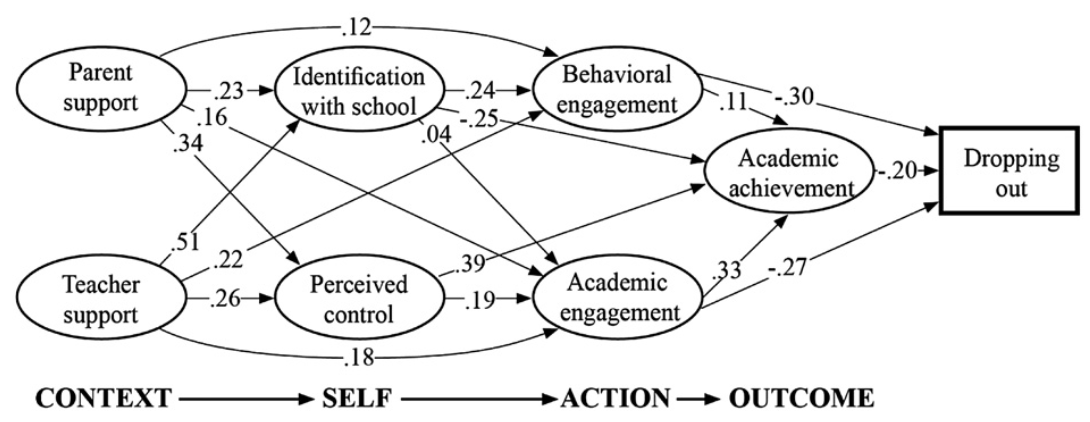
\includegraphics[width=1\textwidth]{Figuras/dropoutmodel}
      \caption{Modelo de interacción sobre el abandono escolar mostrando los factores con significancia mayor a $0.05$\cite{hsdropout}}
    \label{fig:domodel}
\end{figure}

\subsubsection{Una revisión crítica de la literatura sobre la deserción escolar. Año 2013.}

En base al análisis de este documento, que hace un resumen de la literatura disponible, podemos observar que los factores que influyen en la deserción escolar (independiente su grado de influencia) pueden clasificarse en cuatro grandes categorías. 

Estas categorías consideran los factores de cada estudiante, de sus familias, los de su escuela y de la comunidad a la que pertenecen. Los factores de cada categoría se encuentran detallados en el Cuadro~\ref{tab:fact}.

Al analizar estos factores, es posible observar que los efectos observados tienen diferente impacto, es decir, según la literatura, no todos los factores afectan directamente a la predicción de la deserción escolar, y algunos son más importantes que otros. Esto se ve por ejemplo en los factores demográficos, donde el género, raza o etnia y si los estudiantes son inmigrantes o no generan resultados no concluyentes y no es posible definir su influencia.
\cuadro{fact}

\subsubsection{Aplicación de minería de datos en la detección de patrones para detectar el fracaso escolar en Colombia.}

El objetivo de esta literatura es lograr identificar patrones del abandono escolar en estudiantes de la Universidad de Nariño de Colombia utilizando minería de datos. Se utilizaron bases de datos sobre los alumnos admitidos en la primera mitad del 2004 y el segundo semestre 2006, y mediante árboles de decisión se entregó soporte a las decisiones de la universidad.

Los atributos estudiados para este trabajo se presentan en el Cuadro~\ref{tab:attrcol}, y los resultados obtenidos mediante el árbol de decisión se muestran en el Cuadro~\ref{tab:treecol}.
\cuadro{attrcol}
\cuadro{treecol}
De este documento se puede concluir que las reglas que se muestran en el Cuadro~\ref{tab:treecol} generadas por el árbol de decisión son consistentes con la realidad observada y la teoría que hay de fondo con los resultados del árbol de decisión, y que, por tanto, el modelo predictivo es capaz de apoyar la toma de decisiones al desentrañar los factores que se evidencia el abandono para crear planes de retención y mitigación de la deserción. Se hace énfasis en que una de las mayores dificultades está en la calidad de los datos y que existen varios atributos poco útiles.

\subsection{Costo de oportunidad}
Una última arista a considerar en esta revisión bibliográfica son aquellos documentos en los cuales se analiza el costo de oportunidad de dejar la educación. Debido a que no se encontró literatura referente al contexto Chileno, lo que se presenta a continuación está contextualizado en Estados Unidos, cuyos resultados obtenidos permitirán de todas formas generarse una idea en cuanto al costo de oportunidad y cómo influye dejar los estudios.


\subsubsection{El creciente costo de no asistir a la universidad. Año 2014.}
En base a los resultados de una encuesta nacional del \textit{Pew Research Center}, que contempla a 2.002 adultos complementado por un análisis de los datos económicos de la Oficina del Censo de Estados Unidos, se obtiene que los jóvenes con una carrera universitaria actualmente superan a sus pares que no la tienen en cuanto a bienestar económico y logros relacionados con su carrera. Más aún, cuando los adultos jóvenes de hoy se comparan con las generaciones anteriores, se genera una gran disparidad en los resultados económicos entre quienes están graduados de la universidad y quienes solo están graduados de la secundaria (o menos). 

Además de la brecha económica que se encuentra entre los sueldos de quienes poseen un título universitario y quienes no lo poseen, los jóvenes de la generación del milenio que poseen un título universitario plantean que el puesto en que se encuentran actualmente es sólo un trampolín para aspirar a algo mejor, y que consideran que estudiar valió la pena, que es una inversión que ya está dando sus frutos. 

Para examinar el valor de la educación en el mercado laboral actual, el \textit{Pew Research Center} señala la existencia de dos fuentes de datos que son complementarias. La primera es una encuesta representativa a nivel nacional realizada en octubre de 2013, donde se encuestaron 2.002 adultos, de los cuales 630 son de la generación del Milenio, es decir, sus edades están entre 25 y 32 años, edad en que la mayoría de estos adultos jóvenes ya completaron su educación formal y comenzaron su vida laboral. Esta encuesta capturó los puntos de vista de los adultos de hoy con respecto a su educación, su trabajo y sus experiencias en la fuerza laboral.
Además, para medir los resultados económicos de la generación del Milenio y compararlos con otras generaciones de la misma edad, el análisis demográfico de Pew Research Center obtuvo los datos recogidos en la Encuesta de Población Actual del gobierno de los Estados Unidos, la que se lleva a cabo mensualmente. 

En base a la Encuesta de Población Actual, el Pew Research Center definió las siguientes generaciones:
\begin{itemize}
\item La generación del Milenio: quienes nacieron después de 1980, y que en 2013 tienen entre 18 y 32 años.
\item La generación X: quienes nacieron entre 1965 y 1980, y que en 2013 tienen entre 33 y 48 años.
\item La generación Baby Boom tardía: quienes nacieron entre 1955 y 1964, y que en 2013 tienen entre 49 y 58 años.
\item La generación Baby Boom temprana: quienes nacieron entre 1946 y 1954, y que en 2013 tienen entre 59 y 67 años.
\item La generación silenciosa: quienes nacieron entre 1928 y 1945, y que en 2013 tienen entre 68 y 85 años.
\end{itemize}

Actualmente, la generación del milenio es la generación con mayor educación en la historia en la cual la proporción de graduados universitarios ha crecido y el valor de sus títulos se ha incrementado. Sin embargo, en promedio, los ingresos de la generación del milenio (US\$ 35.000) no son muy diferentes a los ingresos de los Boomers tempranos (US\$ 34.883) o la generación X (US\$ 32.173) y sólo un poco más alto que Silents (US\$ 30.982) en edades comparables.

Además se plantea que actualmente, el valor de tener un diploma de secundaria ha disminuido. Mientras que los ingresos de quienes poseen un título universitario subieron, las ganancias de los graduados de la escuela secundaria disminuyeron en más de US\$ 3.000. El \textit{Pew Research Center} ha encontrado que este descenso ha sido lo suficientemente grande como para compensar las ganancias de graduados universitarios. 

El \textit{Pew Research Center} plantea que, si bien tener un título universitario es útil en el mercado laboral actual, esta utilidad varía dependiendo del área principal de estudio, ya que algunos son más relevantes en el trabajo que otros. Por ejemplo, quienes estudiaron ciencias o ingeniería son los más propensos a decir que su trabajo actual está relacionado "muy de cerca" con su carrera universitaria o con el campo de estudios de posgrado.

La encuesta del \textit{Pew Research Center} también indaga entre los graduados de la universidad si se arrepienten de algo relacionado con su carrera y posterior trabajo. Esta lista la encabeza el haber ganado mas experiencia laboral mientras se estudiaba en la universidad, haber estudiado más, haber buscado antes un trabajo y haber escogido un \textit{major} diferente. 


\subsubsection{Mortalidad atribuible a bajos niveles de educación en EEUU. Año 2015.}
Este documento plantea la existencia de disparidades educacionales en la mortalidad de los adultos en EEUU, las que se han ido ampliando a través de los cohortes de nacimiento. 

El tener bajos logros educacionales es un fuerte predictor de la mortalidad prematura en los adultos de EEUU y en muchos otros países. Incluso, las expectativas de vida se han estancado para aquellas personas que poseen menos de la educación secundaria, y va disminuyendo para las mujeres con menos educación. 

Se estima el exceso de mortalidad atribuible a adultos entre 25 y 85 años de EEUU que:
\begin{enumerate}
\item Tienen menos del grado de la escuela secundaria en lugar de un diploma de secundaria o credencial equivalente a la escuela secundaria.
\item Tienen algún estudio universitario en lugar de un título de licenciatura.
\item Tienen algún nivel de educación menor a una licenciatura en lugar de el grado de licenciado.
\end{enumerate}

Para este estudio se utilizan las Encuestas Nacionales de Salud entre 1986-2004, vinculado a un Archivo de Mortalidad hasta el 2006, para estimar las tasas de mortalidad por nivel educativo y cohorte de nacimiento.
Las variables utilizadas incluyen todas las causas de mortalidad. Las categorías educacionales son menos que secundaria, secundaria completa, estudio universitario sin licenciatura, licenciado, y estudios post licenciatura. Raza/etnia y género también son considerados. 
Se utiliza un modelo complementario de supervivencia para tiempo discreto para estimar las tasas de mortalidad. 
Para estimar la mortalidad atribuible al bajo nivel educativo, primero se calcula el número de muertes esperadas al multiplicar las tasas de mortalidad estimadas (tasas de mortalidad específicas y raza ajustados por edad y sexo, por nivel educativo para el 1925, 1935, y 1945 cohortes de nacimiento), con la distribución de los logros educativos, por edad y sexo, de la población de Estados Unidos 2010. La población 2010 ofrece una distribución actual de la educación entre los adultos estadounidenses, que es utilizada para considerar el impacto de las crecientes disparidades educativas en la mortalidad en la mortalidad atribuible. Se estima la población de Estados Unidos de 2010 en base a las Encuestas Nacionales de Salud. Se reúnen las encuestas de 2009, 2010, y 2011 para asegurar estimaciones estables mediante la educación, la edad, el sexo y la raza, y el peso del número de personas a la población censada por el Censo 2010. Se excluyen adultos nacidos en el extranjero. Finalmente, se resta el número estimado de muertes al dar los miembros de algunos grupos educativos las tasas de mortalidad más bajas de aquellos con los niveles más altos de educación.

Los resultados obtenidos muestran que los adultos de entre 25 y 85 años de edad en la población de EEUU 2010 experimentaron las disparidades educativas en la mortalidad observada en la cohorte de 1945, 145.243 muertes pueden atribuirse a las personas que tienen menos de un alto grado de la escuela en lugar de un diploma de secundaria, 110.068 muertes pueden atribuirse a las personas que tienen alguna educación superior en lugar de un título de licenciatura, y 554.525 muertes pueden atribuirse a las personas que tienen cualquier cosa menos que un grado de bachillerato en lugar de un título de licenciatura. Aumento de las disparidades educativas entre los cohortes 1925 y 1945 da como resultado una duplicación de la mortalidad atribuible. La mortalidad atribuible a que tiene menos de un diploma de secundaria es proporcionalmente similar entre las mujeres y los hombres y entre los negros y los blancos no hispanos, y es mayor para la enfermedad cardiovascular que para el cáncer.

Un mayor nivel de educación se asoció inversamente con la mortalidad de los adultos de Estados Unidos a través de mecanismos que incluyen mayores ingresos y estatus social, el desarrollo cognitivo mejorado, una mejor adherencia a los tratamientos médicos, los comportamientos más saludables, y la mejora de las conexiones sociales y el bienestar psicológico.

Se concluye que la mortalidad atribuible al bajo nivel de educación es comparable en magnitud a la mortalidad atribuible a las personas ex fumadores. La investigación existente sugiere que una parte sustancial de la asociación entre la educación y la mortalidad es causal. Por lo tanto, las políticas que aumentan la educación podrían reducir significativamente la mortalidad de adultos.

\subsection{Metodologías de minería de datos}

La cantidad de datos ha ido aumentando de forma exponencial debido a los avances en la tecnología de la computación necesitando que la búsqueda de conocimiento sea de forma automatizada.\cite{datamining2010}

La minería de datos es un proceso que se ideó pensando en descubrir información valiosa dentro de una gran cantidad de datos\footnote{Para este trabajo definimos datos como información textual o numérica con alguna estructura dada} como flujo de entrada y nos entrega conocimiento.\footnote{Esto es una analogía a la industria de la minería donde se extrae los minerales rocosos donde una parte de esta es valiosa}

La minería de datos, tal como es posible observar en la Figura\ref{fig:datamining}, tiene como finalidad generar conocimiento  valioso a partir de un conjunto de datos, la que luego es utilizada para la toma de decisiones o para la comprensión de un fenómeno, y se realiza a través de diferentes tareas que se pueden realizar con los diferentes algoritmos disponibles que los señalaremos posteriormente.

\begin{figure}[H]
  \centering
    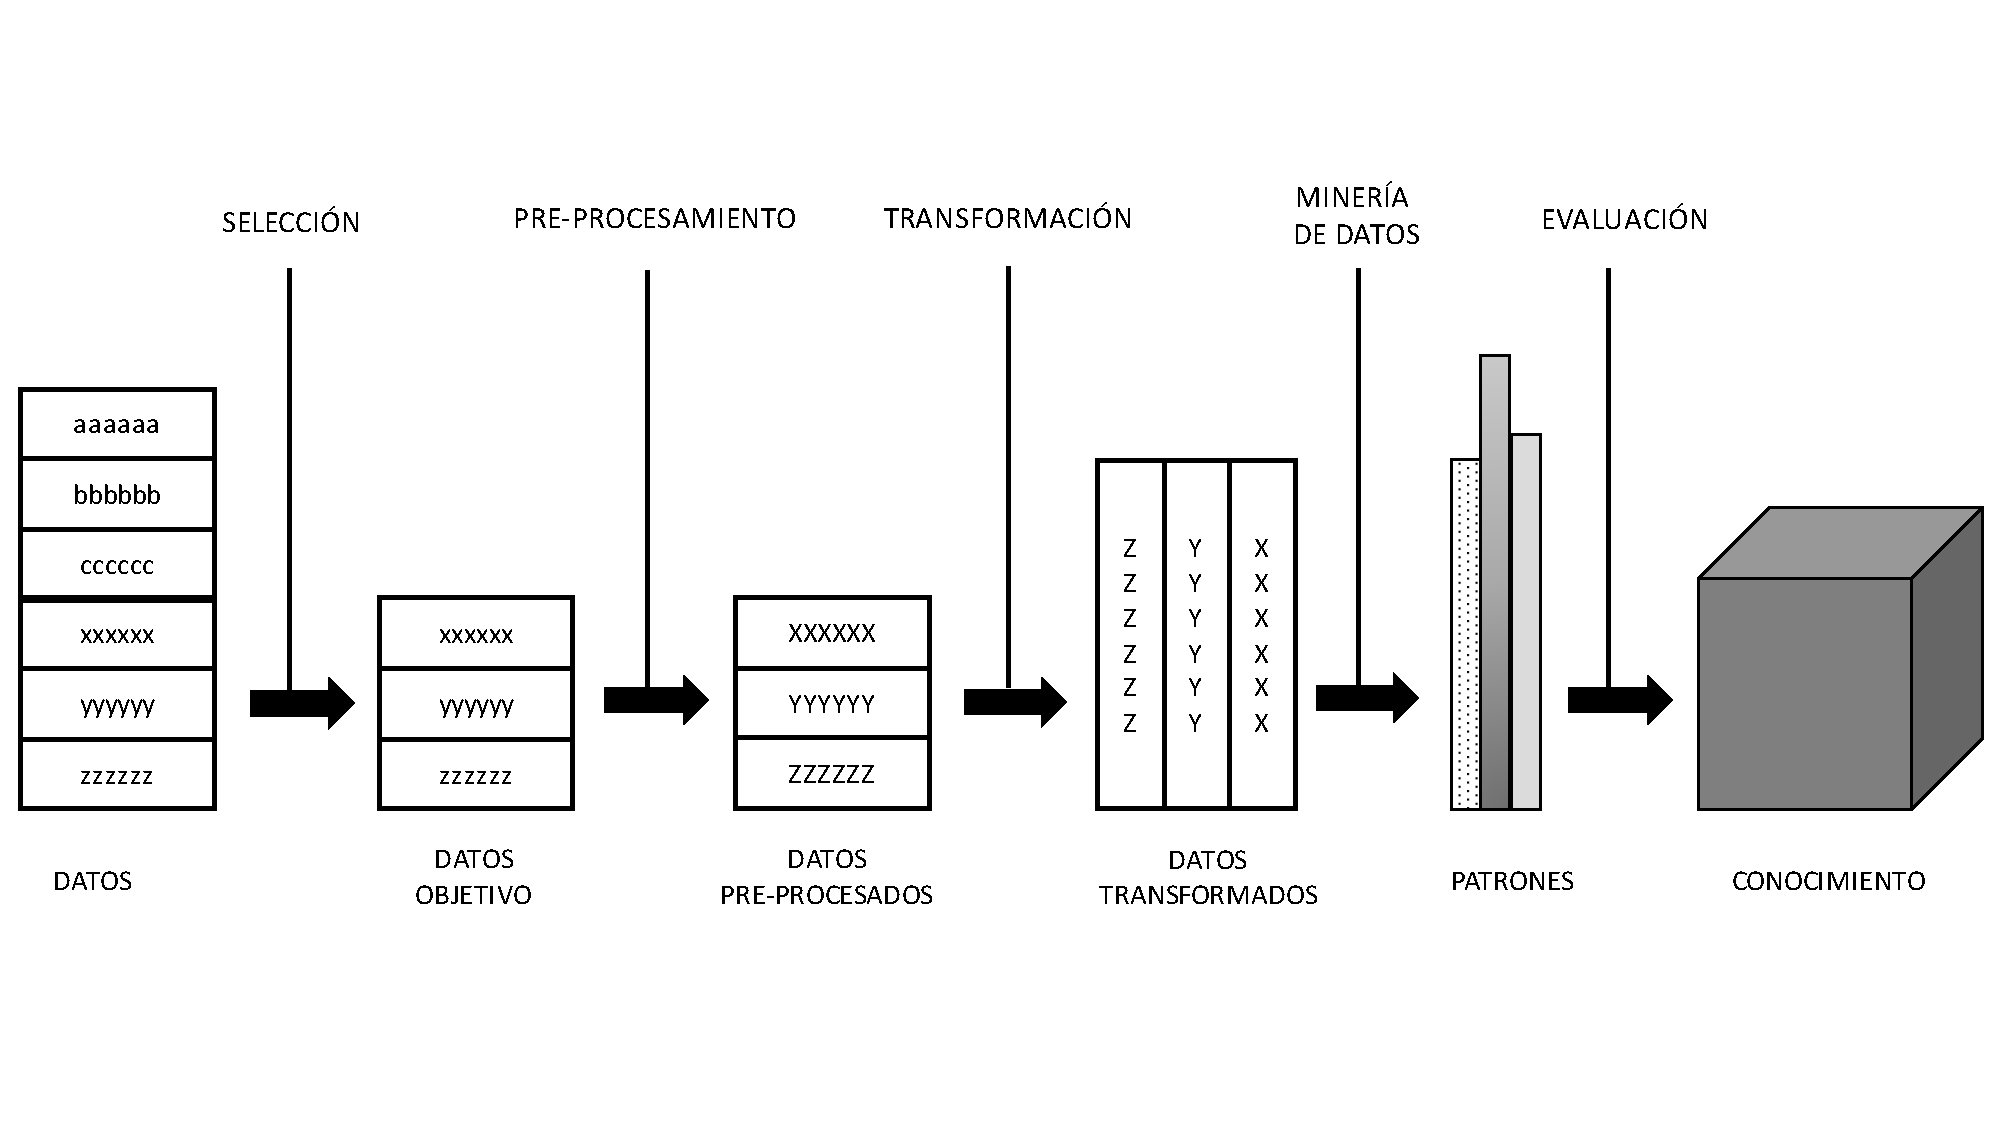
\includegraphics[width=0.9\textwidth]{Figuras/DM}
      \caption{Proceso de Minería de Datos}
    \label{fig:datamining}
\end{figure}

Para realizar minería de datos se han establecido diferentes metodologías para asegurar un resultado coherente con lo que se busca obtener. Existen diferentes metodologías que serán mencionadas y descritas brevemente a continuación.

\subsubsection{KDD}
La metodología \textit{Knowledge Discovery in Databases}\cite{usamafay} o Proceso de Extracción del Conocimiento, tal como su nombre lo dice, es un proceso no trivial de descubrimiento de conocimiento e información potencialmente útil dentro de los datos contenidos en algún repositorio de información (cita de Han, J.; Kamber M. (2001). Data Mining: Concepts ans Techniques. Morgan Kaufmann Publishers, USA.). 
Es un proceso iterativo que explora de forma exhaustiva altos volúmenes de datos con el fin de determinar relaciones. De esta manera es posible extraer información de calidad que se puede utilizar para generar modelos con los datos.

\begin{figure}[H]
  \centering
    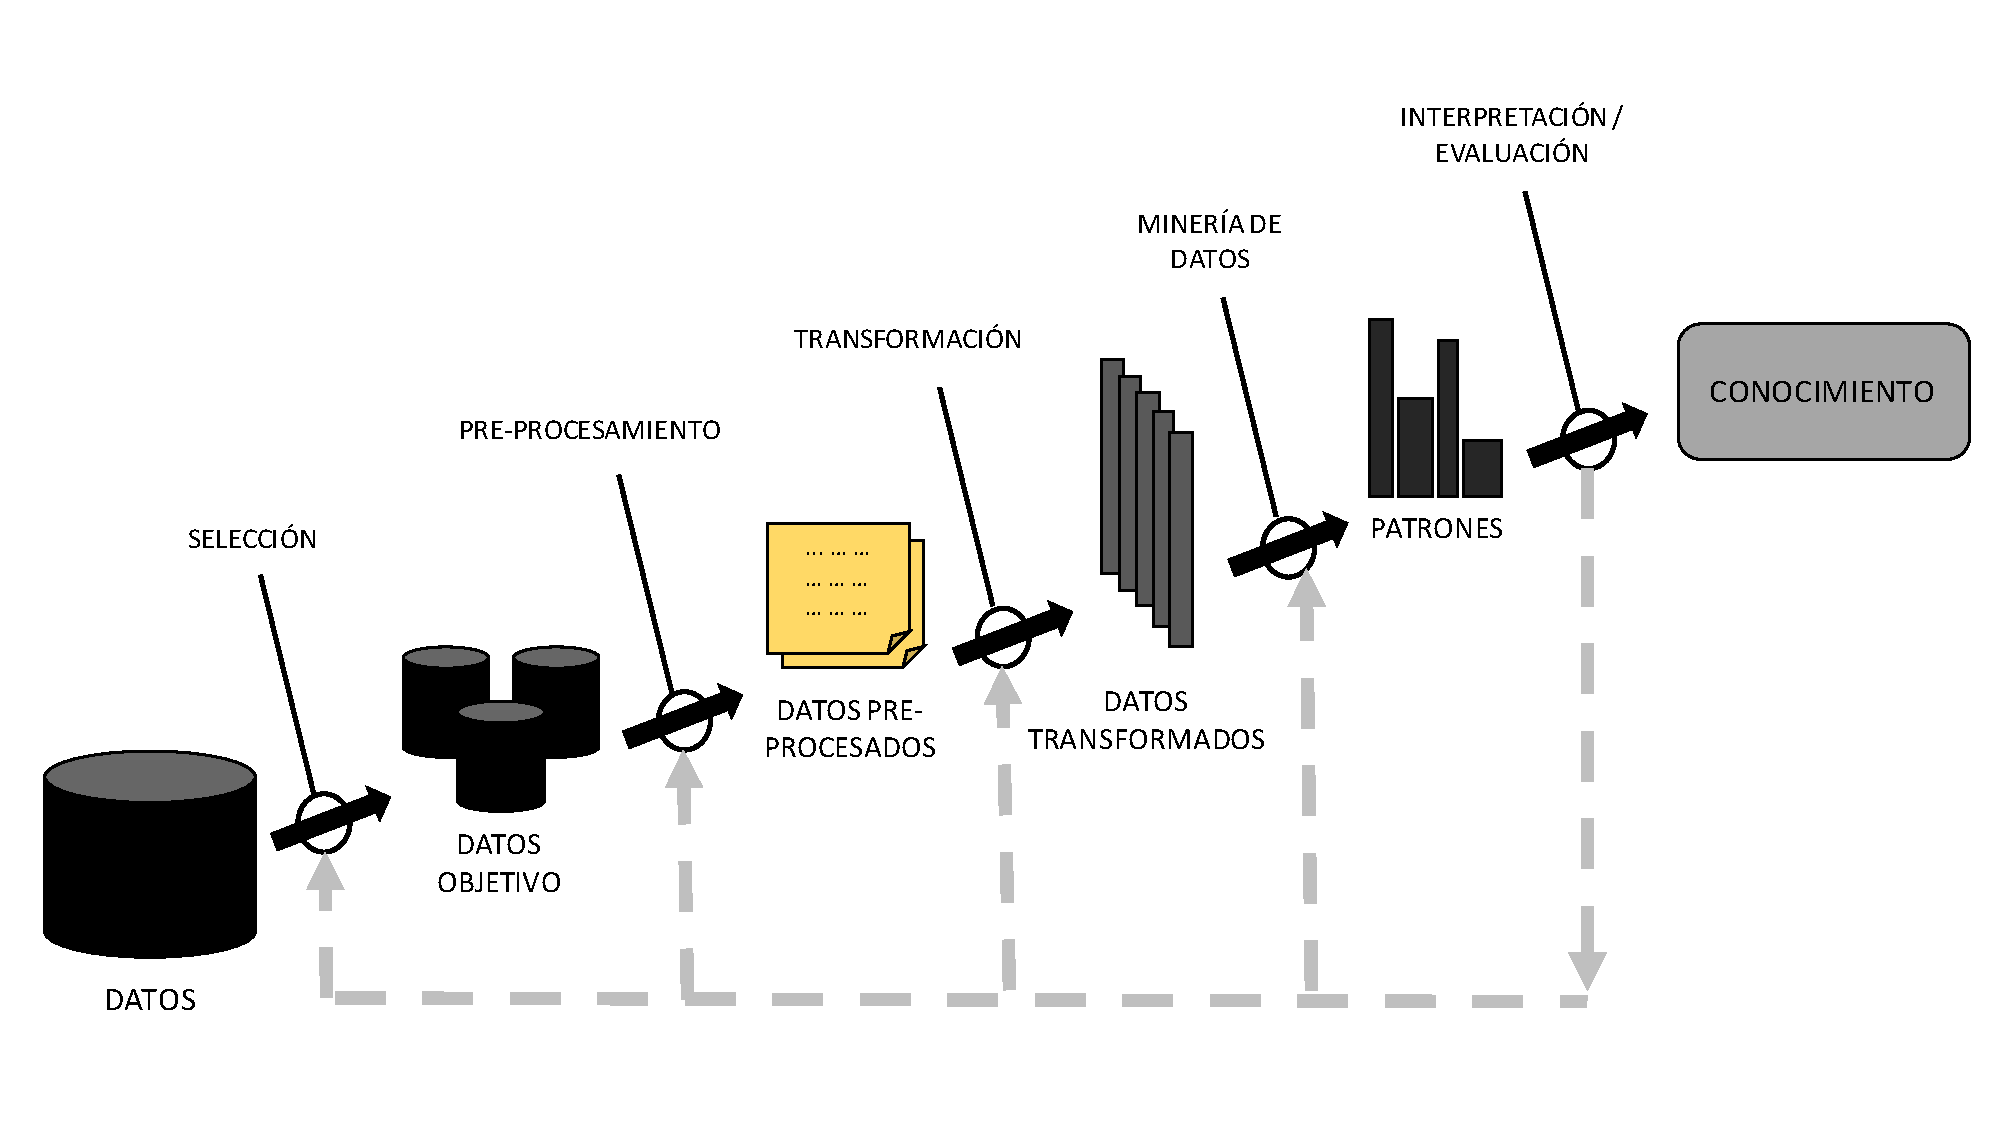
\includegraphics[width=0.9\textwidth]{Figuras/KDD}
      \caption{Etapas de la metodología KDD}
    \label{fig:kdd}
\end{figure}

Como muestra la Figura~\ref{fig:kdd}, el proceso de extracción del conocimiento consta de cinco etapas:
\begin{description}
  \item[1. Selección de Datos:] se determinan las fuentes de datos y el tipo de información a utilizar, es cuando los datos relevantes para el análisis son extraídos de la o las fuentes de datos.
  \item[2. Pre-Procesamiento:] se procede a preparar y limpiar los datos extraídos desde las distintas fuentes de datos seleccionadas anteriormente. Este paso es fundamental para las fases posteriores.Para manejar datos faltantes, inconsistentes o que estén fuera de rango se utilizan diversas estrategias con el fin de obtener una estructura de datos adecuada para su posterior transformación.
  \item[3. Transformación:] consiste en el tratamiento preliminar de los datos, transformando y generando nuevas variables con una estructura de datos apropiada a partir de las ya existentes. Se realizan operaciones de agregación o normalización, consolidando los datos de una forma necesaria para la fase siguiente. 
  \item[4. Minería de Datos:] consiste en el modelamiento propiamente tal, para lo que se aplican métodos inteligentes con el fin de extraer patrones desconocidos, válidos, nuevos, potencialmente útiles y comprensibles y que están "ocultos" en los datos.
  \item[5. Interpretación y Evaluación:] finalmente se identifican los patrones obtenidos y que son realmente interesantes, además de evaluar los resultados obtenidos.
\end{description}

\subsubsection{SEMMA}
La metodología SEMMA, acrónimo de \textit{Sample, Explore, Modify, Model, Assess}, se define como un proceso de selección, exploración y modelamiento de grandes cantidades de datos para descubrir patrones de negocios desconocidos. 

\begin{figure}[H]
  \centering
    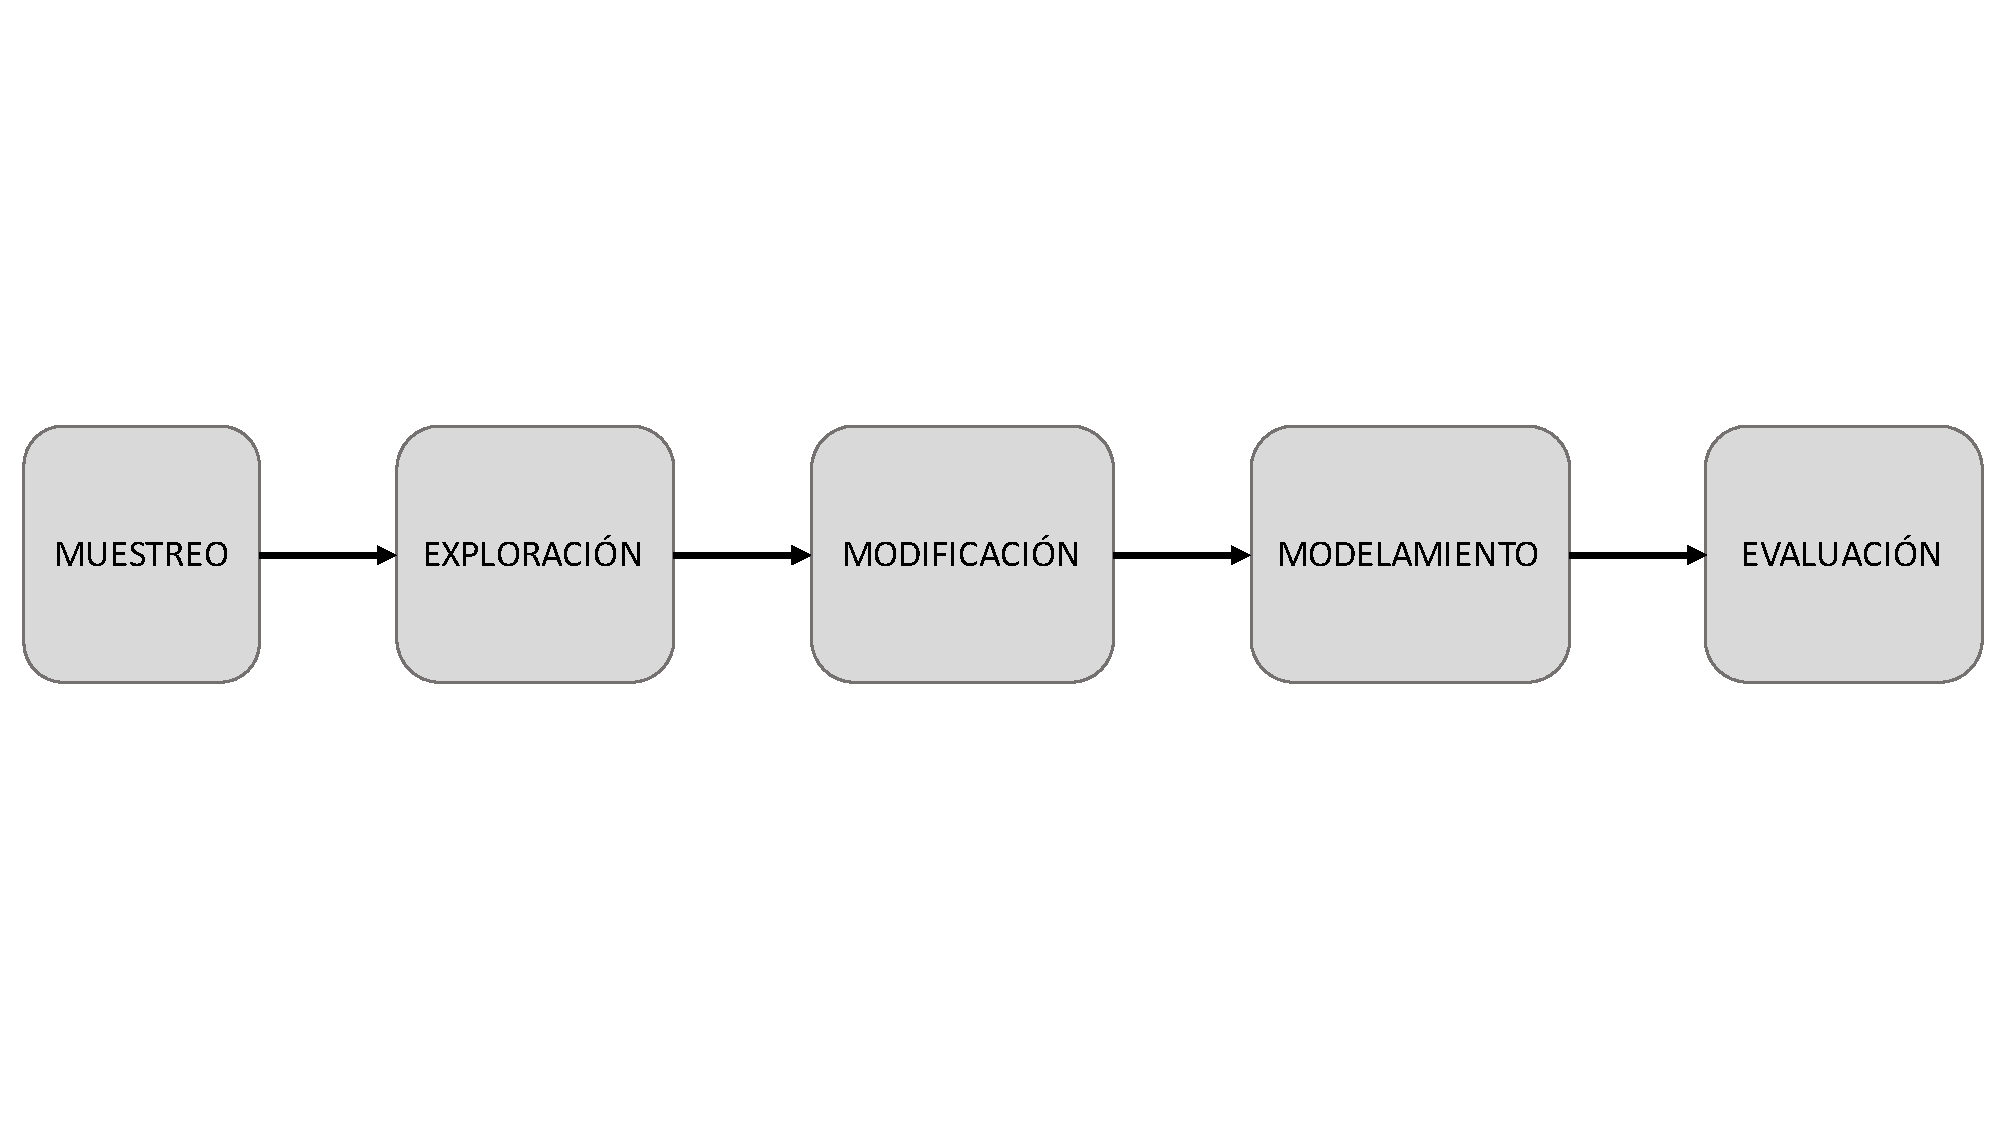
\includegraphics[width=0.9\textwidth]{Figuras/SEMMA}
      \caption{Etapas de la metodología SEMMA.}
    \label{fig:semma}
\end{figure}

En la Figura~\ref{fig:semma} es posible observar que esta metodología consta de cinco etapas:
\begin{description}
  \item[1. Muestreo:] es la etapa inicial, en la cual se procede a preparar los datos para su posterior exploración. En esta etapa es común la utilización del nodo de partición (especialmente si se quiere realizar árboles de decisión o redes neuronales). 
  \item[2. Exploración:] en esta etapa, como lo dice su nombre, se procede a explorar los datos, por lo que es una de las más trabajosas. Se tiene un nodo\footnote{Un nodo multigráfico (o multiplot) es un proceso de minería de datos que permite explorar gráficamente grandes volúmenes de datos para luego crear gráficos de barras, histogramas y gráficos de dispersión con el fin de poder visualizar los datos que se tienen de forma más simple.} que permite explorar gráficamente los datos y otro de selección de variables que permite eliminar aquellos datos de entrada que no tienen relación con la variable objetivo, inclusive se puede realizar un análisis de conglomerados o una segmentación.
  \item[3. Modificación:] en esta etapa el foco es la selección y transformación de variables y datos que servirán para la posterior construcción de modelos. Entre otras tareas, destaca la reducción de dimensión y la imputación de datos perdidos o anómalos.
  \item[4. Modelamiento:] en esta etapa se procede a la selección de modelos. Esta elección depende esencialmente de los datos y variables que se tienen, y de obtener modelos fácilmente entendibles. Entre los modelos está la regresión, la regresión logística, árboles de decisión, análisis factorial discriminante, redes neuronales, entre otros. Se puede aplicar más de uno a la vez, para luego comparar los resultados obtenidos.
  \item[5. Evaluación:] etapa final en la cual se procede a comparar los modelos aplicados y los resultados que se obtienen de ellos. 
\end{description}
%[cita]

\subsubsection{CRISP-DM}
La metodología CRISP-DM o \textit{Cross-Industry Standard Process for Data Mining} es un estándar para los proyectos de minería de datos que incluye un modelo y una guía, estructurados en fases que pueden ser bidireccionales, es decir, al desarrollar una fase es posible revisar parcial o totalmente las anteriores. 

\begin{figure}[H]
  \centering
    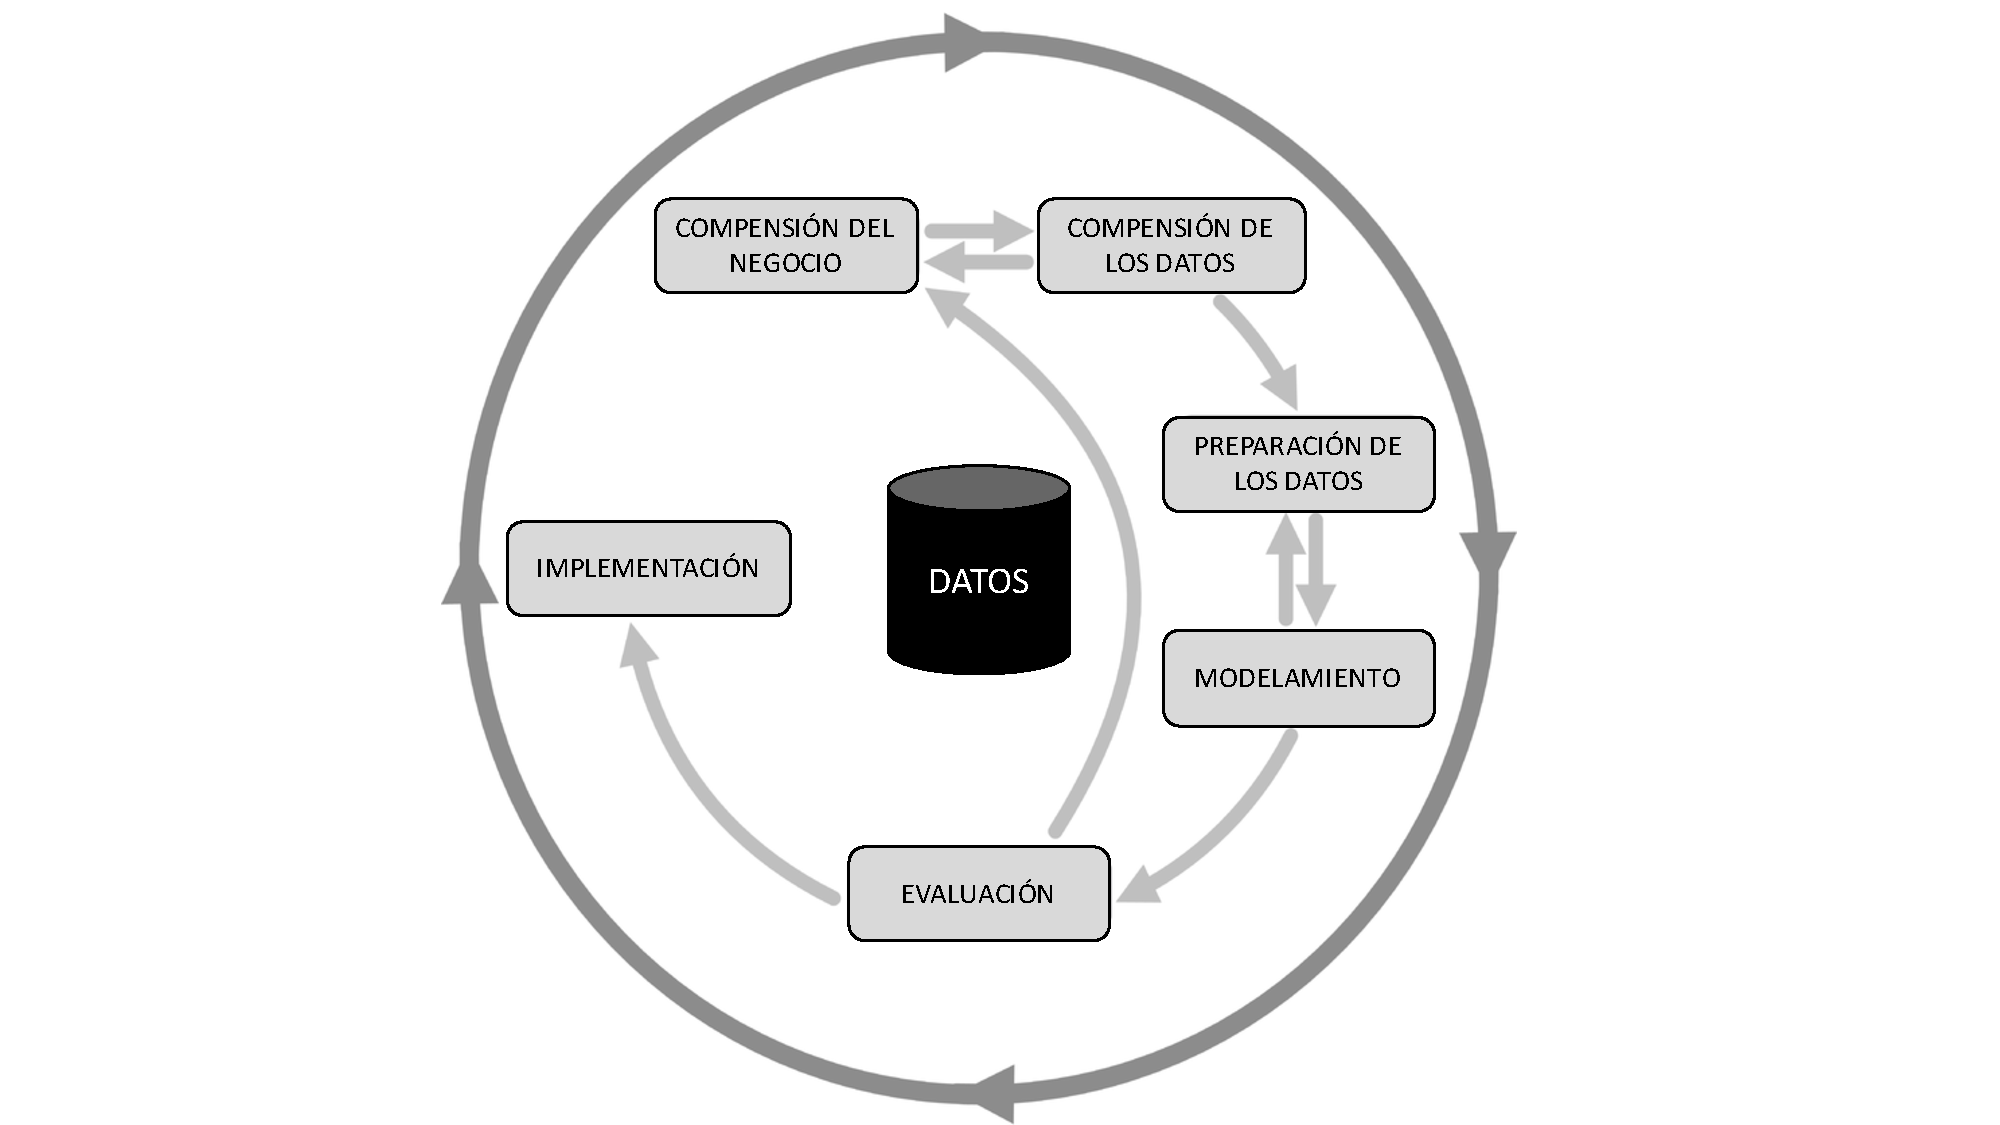
\includegraphics[width=0.99\textwidth]{Figuras/CRISP}
      \caption{Etapas de la metodología CRISP-DM.}
    \label{fig:crisp}
\end{figure}

Como es posible observar en la Figura~\ref{fig:crisp}, esta metodología estructura el proceso en seis fases cuya sucesión no es necesariamente rígida. Cada fase se descompone en varias tareas generales de segundo nivel. Las tareas generales se proyectan a tareas específicas, pero en ningún momento se propone como realizarlas. Es decir, CRISP-DM establece un conjunto de tareas y actividades para cada fase del proyecto pero no especifica cómo llevarlas a cabo.\cite{josegallardo}

Las fases son: 
\begin{description}
  \item[1. Comprensión del Negocio:] fase inicial cuyo objetivo es la comprensión de los objetivos y requisitos del cliente, para luego convertir este conocimiento en objetivos técnicos y en un plan de proyecto. 
  \item[2. Comprensión de los Datos:] el objetivo es establecer un primer contacto con el problema, por lo que requiere una recolección inicial de datos para familiarizarse con ellos, identificar su calidad y establecer las relaciones más evidentes para luego definir las primeras hipótesis. Esta fase junto a las próximas dos, son las que demandan el mayor esfuerzo y tiempo en un proyecto de minería de datos.
  \item[3. Preparación de los Datos:] una vez efectuada la recolección inicial de datos, se procede a su preparación para adaptarlos a las técnicas de minería de datos que posteriormente se utilicen. Este proceso incluye tareas generales de selección de datos a los que se va a aplicar una determinada técnica de modelado, limpieza de datos, generación de variables adicionales, integración de diferentes orígenes de datos y cambios de formato.
  \item[4. Modelamiento:] se seleccionan las técnicas de modelado apropiadas para el proyecto. Esta selección se debe realizar en función de los siguientes criterios: que sea apropiada al problema, disponer de los datos adecuados, cumplir con los requisitos del problema, tiempo adecuado para obtener un modelo y conocimiento de la técnica. 
  \item[5. Evaluación:] se procede a la evaluación del modelo considerando el cumplimiento de los criterios de éxito del problema. Además, debe considerarse que la fiabilidad calculada para el modelo se aplique sólo para los datos sobre los que se realizó el análisis. Es preciso revisar el proceso, teniendo en cuenta los resultados obtenidos, para poder repetir algún paso anterior, en el que se haya posiblemente cometido algún error. Es importante considerar que se pueden emplear múltiples herramientas para la interpretación de los resultados. Luego, si el modelo generado es válido en función de los criterios de éxito establecidos en la fase anterior, se procede a la explotación del modelo.
  \item[6. Implementación:] luego de que el modelo ha sido construido y validado, se procede a transformar el conocimiento obtenido en acciones dentro del proceso de negocio.
\end{description}
\section{Paradigmas}
En la sección anterior se presentaron los documentos más importantes que avalan los objetivos de este estudio. 
En base a ellos es posible notar que hay ciertas visiones y deducciones que se presentan, de diferentes formas, en más de un documento. La finalidad de esta sección es analizar algunos de estos puntos en común, a los que llamaremos paradigmas, ya que formarán parte del conjunto de conocimientos que forman una visión del fenómeno de la deserción escolar en Chile. Estos permitirán determinar las direcciones en que se desarrollará este estudio y establecer sus límites. 

\subsection{Deserción escolar como un proceso}
De la literatura revisada y mencionada, se desprende que la deserción escolar en Chile es considerada como un proceso de alejamiento y abandono paulatino de un espacio cotidiano, que en este caso es el establecimiento educacional, y no como un resultado.

Este proceso no es posible explicarlo sin considerar elementos de distintas índoles que requieren, por su naturaleza, un análisis integral e integrado que comience por la comprensión de la multiplicidad de causas que los originan. Es por esto que al hablar del proceso de deserción escolar no existe un camino único, y los factores que en esto inciden se presentan de diferentes maneras.

De lo anterior deriva el hecho que la deserción es un proceso distinto para cada uno de los alumnos que finalmente deciden dejar el sistema educacional, pero en base a los estudios es posible afirmar que se van generando patrones en los cuales existen factores en común. 

\subsection{Tres niveles de factores que explican el proceso de deserción escolar en Chile}
Otro punto importante a considerar luego de la revisión bibliográfica, y del análisis de la deserción como un proceso, son los factores que generan esta situación y el origen de estos. El Cuadro~\ref{tab:resumen} presenta un resumen de los factores relevantes encontrados en la literatura revisada. 

\cuadro{ResumenFactores}

Es importante mencionar que en un fenómeno tan complejo como la deserción escolar, ningún elemento o factor explicativo considerado por si sólo tiene el peso suficiente para dar cuenta por completo de esto. 

En base a los documentos ya mencionados y resumidos en el Cuadro~\ref{tab:resumen}, es posible tener una idea previa con respecto a los factores que influyen en la decisión de desertar. También, es posible definir preliminar tres grupos de factores según de dónde estos provienen, del contexto del establecimiento o intraescolares, factores personales del alumno y factores provenientes de su ambiente familiar. Estos se presentan a grandes rasgos a continuación. 

\subsubsection{Factores intraescolares}
Los factores intraescolares son aquellos que caracterizan al establecimiento educacional al que asiste el alumno, como si este es municipal o particular subvencionado, el ambiente considerando violencia, consumo y tráfico de drogas, un mal comportamiento en el colegio, problemas graves con compañeros y profesores, dónde está ubicado, la cantidad de matrículas, entre otros.  Además se considera aquí todo lo relativo a los docentes; como su nivel de educación, los títulos que poseen, la cantidad de horas lectivas que realizan, en cuántos colegios realizan clases, los años de trayectoria que llevan, entre otros. 
\subsubsection{Factores personales}
Los factores personales son aquellos relacionados con la vida del alumno y su estilo de vida. Están compuestos por características del individuo que no forman parte de una condición o estado de salud, sino que con su personalidad y la forma en que se desenvuelven en el día a día. 
Dentro de estos factores se encuentra el rendimiento del alumno, su tasa de asistencia a clases, problemas conductuales, repitencias, expulsiones, sobreedad, traslados. Además se considera cuán cerca vive el alumno del colegio y la oferta educacional de las cercanías a su hogar. 
\subsubsection{Factores familiares}
Los factores familiares de un alumno son aquellos relacionados con su hogar y ambiente familiar, dentro de los cuales se encuentra la situación socioeconómica de la familia del alumno, su contexto familiar, la escolaridad de los padres, la pobreza y la marginalidad, la búsqueda de trabajo, el embarazo adolescente, la disfuncionalidad familiar, el consumo de drogas, las bajas expectativas de la familia con respecto a la educación, el capital cultural y apoyo entre otros.

\section{Nuevos retos}
Al momento de analizar la literatura existente es posible notar que se generan ciertos retos dado que no existe una metodología única mediante la cual se estudie y analice la deserción escolar en nuestro país. 
Por otro lado, estos retos también se hacen parte de nuestro estudio, ya que para lograr los objetivos planteados en el primer capítulo son obstáculos en los que se debe trabajar. 
\subsection{Información estandarizada}
Un primer reto que es posible notar es la obtención de información y datos de diferentes fuentes y con diferentes métodos a diferentes muestras. 
Es importante tener información actualizada y disponible con el fin de facilitar su utilización. 
\subsection{Gestión de la información}
Gestionar la información previamente estandarizada resulta primordial para la generación de conocimientos. Este proceso de creación de conocimientos implica determinar la información que sea precisa, recoger y analizar la información, registrarla y recuperarla cuando sea necesaria con el fin de utilizarla y divulgarla. 
El objetivo de realizar este proceso es garantizar la integridad, disponibilidad y confidencialidad de la información para las autoridades 
\subsection{Ampliar prototipo de alerta temprana al país}
El último reto nace específicamente de este estudio, el cual tiene como objetivo crear un prototipo de alerta temprana de la deserción escolar para los establecimientos municipales y particulares subvencionados de la región Metropolitana, aspirando posteriormente a su ampliación a todas las regiones del país. Para lograr esto, es necesario que los dos puntos anteriores estén cubiertos, con el fin del facilitar el proceso.

\section{Conclusiones}
En este capítulo se analizaron los documentos principales relacionados con la deserción escolar en Chile. Existen dos grandes grupos de estudios con respecto al tema, estudios cuantitativos que dan a conocer la deserción escolar en cifras, y los cualitativos que buscan explicar estas cifras mediante el análisis de diferentes factores. De aquí se desprenden dos grandes paradigmas que guiarán este estudio. El primero es la deserción escolar como un proceso, y el segundo son las tres esferas que interactúan y van generando este proceso. 

Se encuentra también un grupo de estudios internacionales en los cuales se analizan temas sobre la predicción del éxito académico. En Colombia se utilizó minería de datos para detectar patrones del fracaso escolar y posterior a esto, mediante árboles de decisiones, se concluye que el modelo predictivo es capaz de encontrar los factores que generan esta situación. 

Luego, con respecto al costo de oportunidad, se presentan dos documentos relacionados con el costo de oportunidad de no estudiar, cuyo contexto es EEUU. De estos se puede concluir que, para las generaciones actuales el valor de tener el diploma de secundaria ha disminuido en relación a generaciones anteriores, por lo que para acceder a mejores oportunidades laborales no es necesario solamente terminar los 12 años de escolaridad, sino que obtener un título universitario es prácticamente lo mínimo para abrirse puertas en el mercado laboral. Por otro lado, también se puede concluir que existe un alto costo asociado al hecho de no terminar los estudios, que aumenta cuando se habla de un título universitario y estudios superiores a esto. Además se plantea que los bajos niveles de educación están asociados con altas tasas de mortalidad en adultos, por lo que las políticas que aumentan la educación podrían reducir la mortalidad.

Finalmente, se presentan las metodologías de minería de datos que son candidatas a guiar este proyecto. 